% !TEX root = recipeUnderstanding.tex


\subsection{Unsupervised Parsing}
\label{basics}
\label{learning}
In this section, we explain the model which we use to discover the activity steps from a video collection given the language and visual atoms. We note the extracted representation of the frame $t$ of video $i$ as $\mathbf{y^{(i)}_t}$. We model our algorithm based on activity steps and note the activity label of the $t^{th}$ frame of the $i^{th}$ video as $z^{(i)}_t$. We do not fix the the number of activities and use a non-parametric approach.

%We start with explaining the notation. As we already defined in the previous sections,

In our model, each activity step is represented over the atoms as the likelihood of including them. In other words, each activity step is a Bernoulli distribution over the visual and language atoms as $\theta_k=[\theta_k^l,\theta_k^v]$ such that $m^{th}$ entry of the $\theta_k^l$ is the likelihood of observing $m^{th}$ language atom in the frame of an activity $k$. Similarly, $m^{th}$ entry of the $\theta_k^v$ represents the likelihood of seeing $m^{th}$ visual atom. In other words, each frame's representation $\mathbf{y^{(i)}_t}$ is sampled from the distribution corresponding to its activity as \mbox{$\mathbf{y^{(i)}_t}|z^{(i)}_t=k \sim Ber(\theta_k)$}. As a prior over $\theta$, we use its conjugate distribution -- \emph{Beta distribution}.

Given the model above, we explain the generative model which links activity steps and frames in Section~\ref{bphmm}.
 %The key idea is each frame is represented via atoms and each activity step is a distribution over atoms hence the atoms are the linkage. We further explain the learning method to fit this model without any supervision in the Section~\ref{gibbs}.
 
   \vskip -2mm
\subsubsection{Beta Process Hidden Markov Model}
\label{bphmm}
  \vskip -2mm
  
For the understanding of the time-series information, Fox et al.~\cite{foxBPHMM} proposed the Beta Process Hidden Markov Models (BP-HMM). In BP-HMM setting, each time-series exhibits a subset of available features. Similarly, in our setup each video exhibits a subset of activity steps.
%It is based on the notion features(\eg activity steps) which can explain the behaviour of a collection of time-series data (\eg video collection).

Our model follows the construction of Fox et al.~\cite{foxBPHMM} and differs in the choice of probability distributions since \cite{foxBPHMM} considers Gaussian observations while we adopt binary observations of atoms. In our model, each video $i$ chooses a set of activity steps through an activity step vector $\mathbf{f^{(i)}}$ such that $f^{(i)}_k$ is $1$ if $i^{th}$ video has the activity step $k$, and 0 otherwise. When the activity step vectors of all videos are concatenated, it becomes an activity step matrix $\mathbf{F}$ such that $i^{th}$ row of the $\mathbf{F}$ is the activity step vector $\mathbf{f^{(i)}}$. Moreover, each activity step $k$ also has a prior probability $b_k$  and a distribution parameter $\theta_k$ which is the Bernoulli distribution as we explained in the Section~\ref{basics}.

In this setting, the activity step parameters $\theta_k$ and $b_k$ follow the \emph{beta process} as;
\vskip -2mm
\begin{equation}
  B|B_0,\gamma,\beta \sim \text{BP}(\beta,\gamma B_o), B=\sum_{k=1}^\infty b_k \delta_{\theta_k}
\end{equation}
where $B_0$ and the $b_k$ are determined by the underlying Poisson process \cite{ibp} and the feature vector is determined as independent Bernoulli draws as $f_{k}^{(i)} \sim Ber(b_k)$. After marginalizing over the $b_k$ and $\theta_k$, this distribution is shown to be equivalent to Indian Buffet Process (IBP)~\cite{ibp}. In the IBP analogy, each video is a customer and each activity step is a dish in the buffet. The first customer (video) chooses a $\text{Poisson}(\gamma)$ unique dishes (activity steps). The following customer (video) $i$ chooses previously sampled dish (activity step) $k$ with probability $\frac{m_k}{i}$,  proportional to the number of customers ($m_k$) chosen the dish $k$, and it also chooses $\text{Poisson}(\frac{\gamma}{i})$ new dishes (activity steps). Here, $\gamma$ controls the number of selected activities in each video and $\beta$ promotes the activities getting shared by videos.

The above IBP construction represents the activity step discovery part of our method. In addition, we need to model the video parsing over discovered steps; these two need to be modeled jointly. We model the each video as an Hidden Markov Model (HMM) over the selected activity steps. Each frame has the hidden state --activity step-- ($z^{(i)}_t$) and we observe the multi-modal frame representation $\mathbf{y^{(i)}_t}$. Since we model each activity step as a Bernoulli distribution, the emission probabilities follow the Bernoulli distribution as $p(\mathbf{y^{(i)}_t}|z^{(i)}_t)=Ber(\theta_{z^{(i)}_t})$.

For the transition probabilities of the HMM, we do not put any constraint and simply model it as any point from a probability simplex which can be sampled by drawing a set of Gamma random variables and normalizing them \cite{foxBPHMM}. For each video $i$, a Gamma random variable is sampled for the transition between activity step $j$ and activity step $k$ if both of the activity steps are included in the video (\ie if $f^i_k$ and $f^i_j$ are both $1$). After sampling these random variables, we normalize them to make transition probabilities to sum to 1. This procedure can be represented formally as
\begin{equation}
  \eta_{j,k}^{(i)} \sim Gam(\alpha+\kappa \delta_{j,k},1), \quad \mathbf{\pi_j^{(i)}} = \frac{\mathbf{\eta^{(i)}_j} \circ \mathbf{f^{(i)}}}{\sum_k \eta^{(i)}_{j,k} f^{(i)}_k},
\end{equation}
where $\kappa$ is the persistence parameter promoting the self state transitions a.k.a. more coherent temporal boundaries, $\circ$ is the element-wise product, and $\pi^i_j$ is the transition probabilities in video $i$ from activity step $j$ to other steps. This model is also presented as a graphical model in Figure~\ref{bphmmo}.
\begin{figure}[h!]
  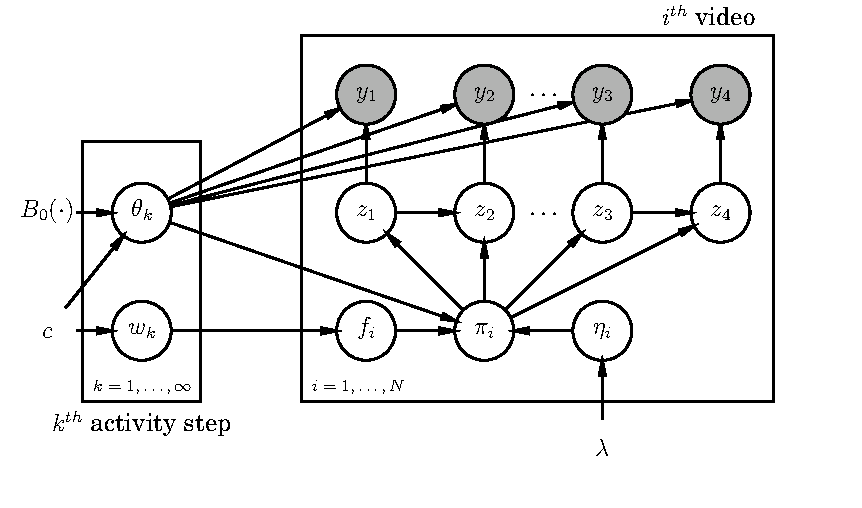
\includegraphics[width=0.5\textwidth]{plate}
  \vspace{-9mm}
  \caption{\textbf{Graphical model for BP-HMM:} The left plate represent the activity steps and the right plate represent the videos. (\ie the left plate is for the activity step discovery and right plate is for parsing.) \emph{See Section~\ref{bphmm} for details.}}
  \vspace{-5mm}
  \label{bphmmo}
\end{figure}


\subsubsection{Gibbs sampling for BP-HMM}
We employ Markov Chain Monte Carlo (MCMC) method for learning and inference of the BP-HMM. We base our algorithms on the MCMC procedure proposed by Fox et al.~\cite{foxBPHMM}. Our sampling procedure composed of two samplers: (1) activity step ($\mathbf{f^{(i)}}$) sampler from the current activity step distributions $\mathbf{\theta_k}$ and multi-modal frame representations $y^{(i)}_k$, (2) and HMM parameter $\mathbf{\eta}$,$\mathbf{\pi}$,$\mathbf{\theta_k}$ sampler from the selected activities $\mathbf{f^{(i)}}$. Intuitively, we iterate over discovering activity steps given the temporal activity labels and estimating activity labels given the discovered activities. We give the details of this sampler in \cite{supp}.
